\chapter{Methodology}
% Chapter 3 - Some important points
%==========================
This Chapter gives some points on writing which was not discussed in the class.

\section{Full Converter}
For full-power conversion either buck, boost, or buck \textendash boost converters can be used \cite{a1}. 
Other, more complex topologies like, e.g., the SEPIC converter are not considered here due to 
their higher system complexity.
The greatest flexibility is given with buck - boost converters Figure (\ref{fig:buckboost}) where
any string current value can be matched by the output currents of the converters.

\begin{figure}[h]
	\begin{center}
	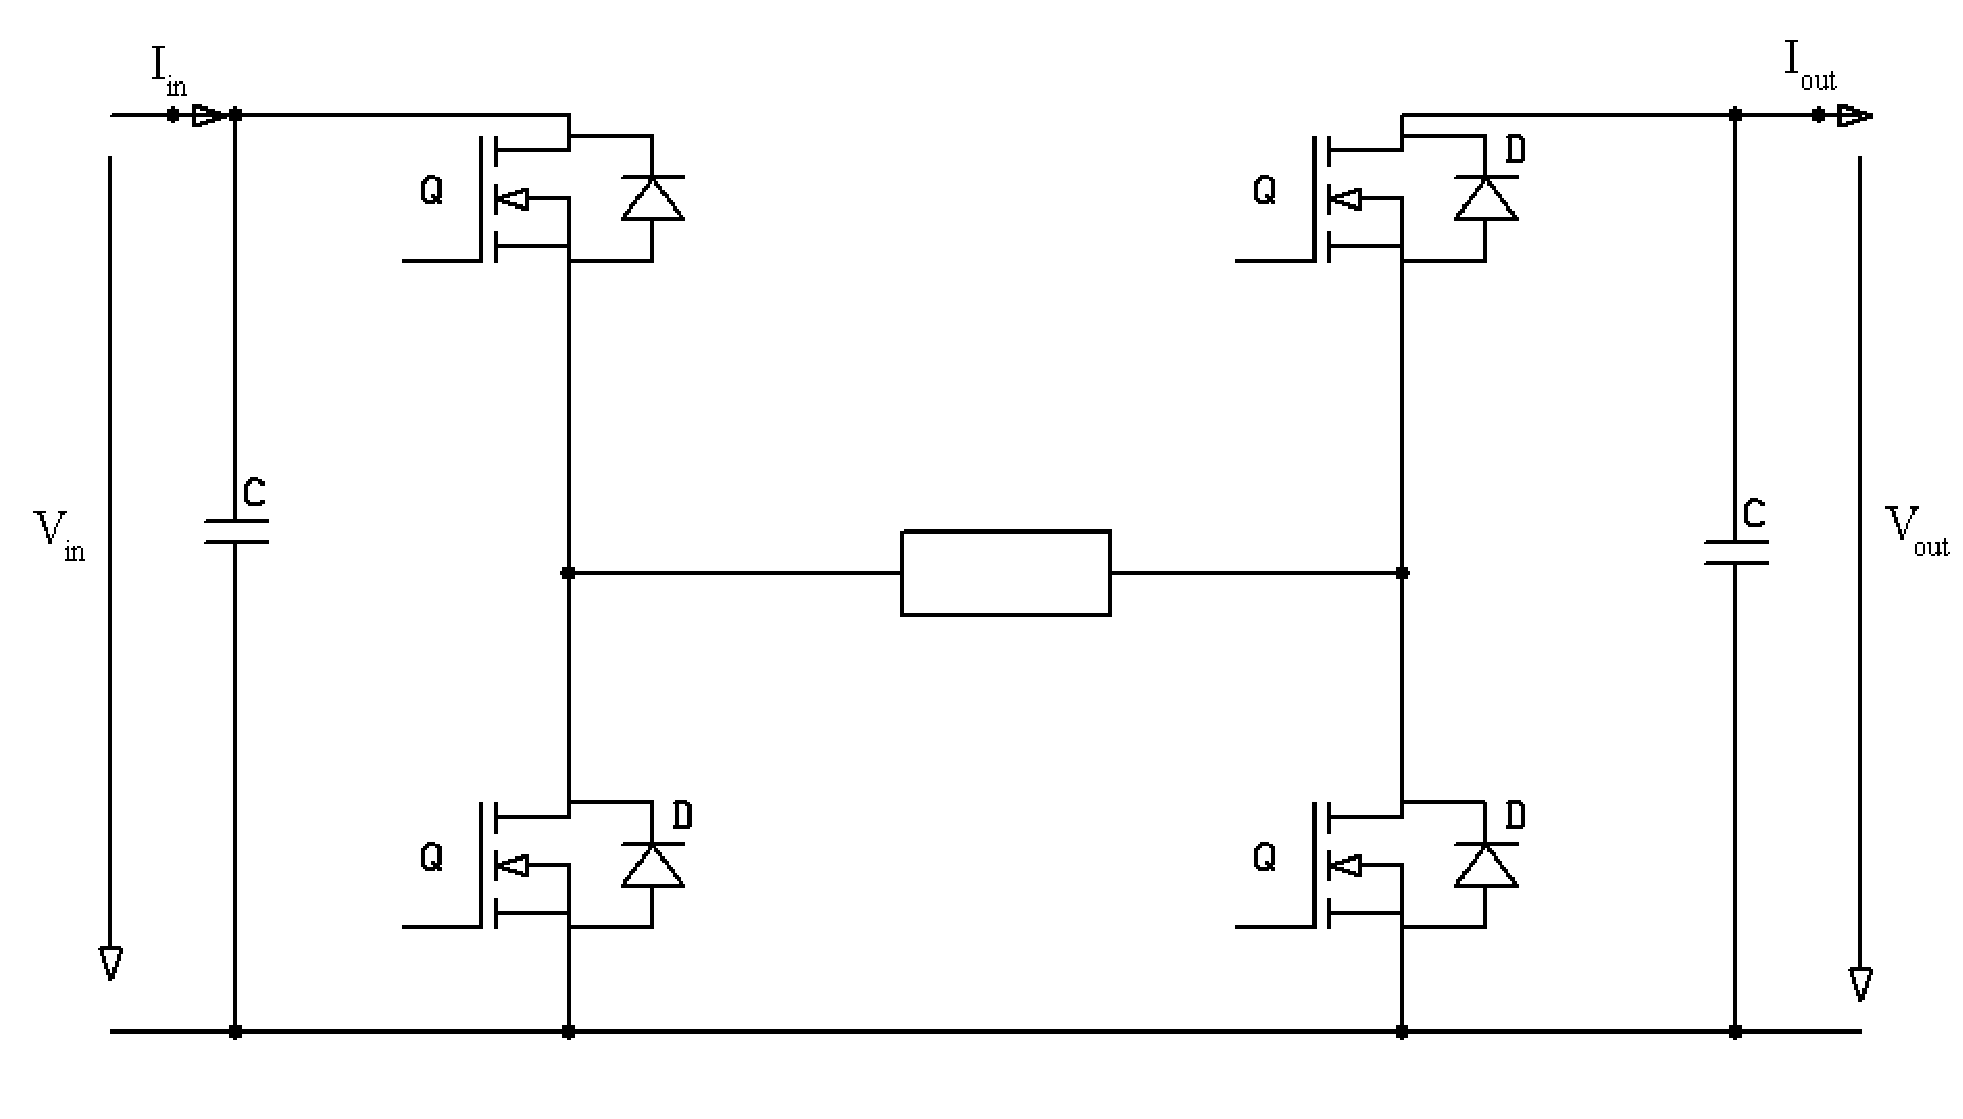
\includegraphics[width=0.5\textwidth]{LiteratureReview/buckboost.pdf}
	\caption{Buck\textendash Boost converter}
	\label{fig:buckboost}
	\end{center}
\end{figure}

Buck \textendash boost converters allow to keep the bus voltage constant since any level of 
string current can be set. Thus, the upper limit of PV panels per string for the buck\textendash boost 
converter concept depends on the maximum output current rating, and the lower limit depends on the 
maximum output voltage rating of the buck\textendash boost converters. In Table (\ref{table:max_minPVpanels}),
the equations for the maximum and minimum numbers of PV panels per string are given for the 
three different full\textendash power converter topologies under the assumption that all panels 
should be able to feed power into the string under a given shading condition which can be 
expressed as $\Delta = \frac{P_{PV,unsh}}{P_{PV,sh}}$ . 

\begin{table}[h]
	\centering
		\begin{center}
		\centering
		\caption{Maximum, Resp. Minimum number of PV panels per string for different MIC topologies} \label{table:max_minPVpanels}
		\end{center}
	\centering
	\begin{tabular}{l|c|c}
	\hline \rule[-2ex]{0pt}{5.5ex} Type & Max. no. of PV panels & Min. no. of PV panels \\ \hline 
	\hline \rule[-2ex]{0pt}{5.5ex} 
   	    Buck &$\frac{V_{BUS}}{P_{PV,MAX}}I_{OUT,MAX}$  & $(\frac{V_{BUS}}{V_{MPP}}\Delta +1$) \\ 
	\hline \rule[-2ex]{0pt}{5.5ex} 
	    Boost &$\frac{V_{BUS}+(\Delta-1)V_{MPP}}{\Delta.V_{MPP}}$  &$(\frac{V_{BUS}}{V_{out,MPP}}-1)\Delta+1$  \\ 
	\hline \rule[-2ex]{0pt}{5.5ex} 
	   Buck-Boost &$\frac{V_{BUS}}{P_{PV,MAX}}I_{OUT,MAX}$  & $(\frac{V_{BUS}}{V_{out,MPP}}-1)\Delta+1$ \\ 
	\hline 
	\end{tabular} 
\end{table}

Here, 
\begin{enumerate}[(i)]
	\item $I_{Out,Max}$ is the maximum output current of the converter
	\item $V_{MPP}$ is the PV panel voltage in a typical MPP
	\item $P_{PV,max}$ is the the maximum output power
\end{enumerate}



\section{Giving references}
An equation, figure or table given in any chapter can be called as follows: (For details refer the .tex file of this chapter). 

Consider (\autoref{table:max_minPVpanels}) and (\autoref{fig:buckboost}) given in Chapter(\ref{chap:app}). Chapter reference can also be 
given as (\autoref{chap:app}). 

Citations can be given as \cite{a2}. Any reference to books can also be noted in the bib file and can be cited as \cite{b1} and proceedings in the form \cite{p1}.


\section{Matrix Equation}
Matrices can be given as in equation (\ref{eq.matrixA}),
\begin{eqnarray}
	\dot x = \mathbf Ax \label{eq.stateeqn}
\end{eqnarray}

where,
\begin{eqnarray}
	\mathbf A = \begin{bmatrix}
	             a_1 & a_2 & a_3 \\
	             b_1 & b_2 & b_3 \\
	             c_1 & c_2 & c_3 \\
	      	    \end{bmatrix} \label{eq.matrixA}
\end{eqnarray}


\section{Figures}

Figures can be grouped and separate captions can be given for each figure as Figure (\ref{fig:subcaption1}), (\ref{fig:subcaption2}) and (\ref{fig:subcaption3}). A caption can also be given for the group as Figure (\ref{fig:maincaption}). See the .tex file for details. 

%Figure - 3D icosahedral quasicrystal- Al-Pd-Mn
%====================================
\begin{figure}
    \centering
    \begin{subfigure}[b]{0.48\textwidth}
        \centering
        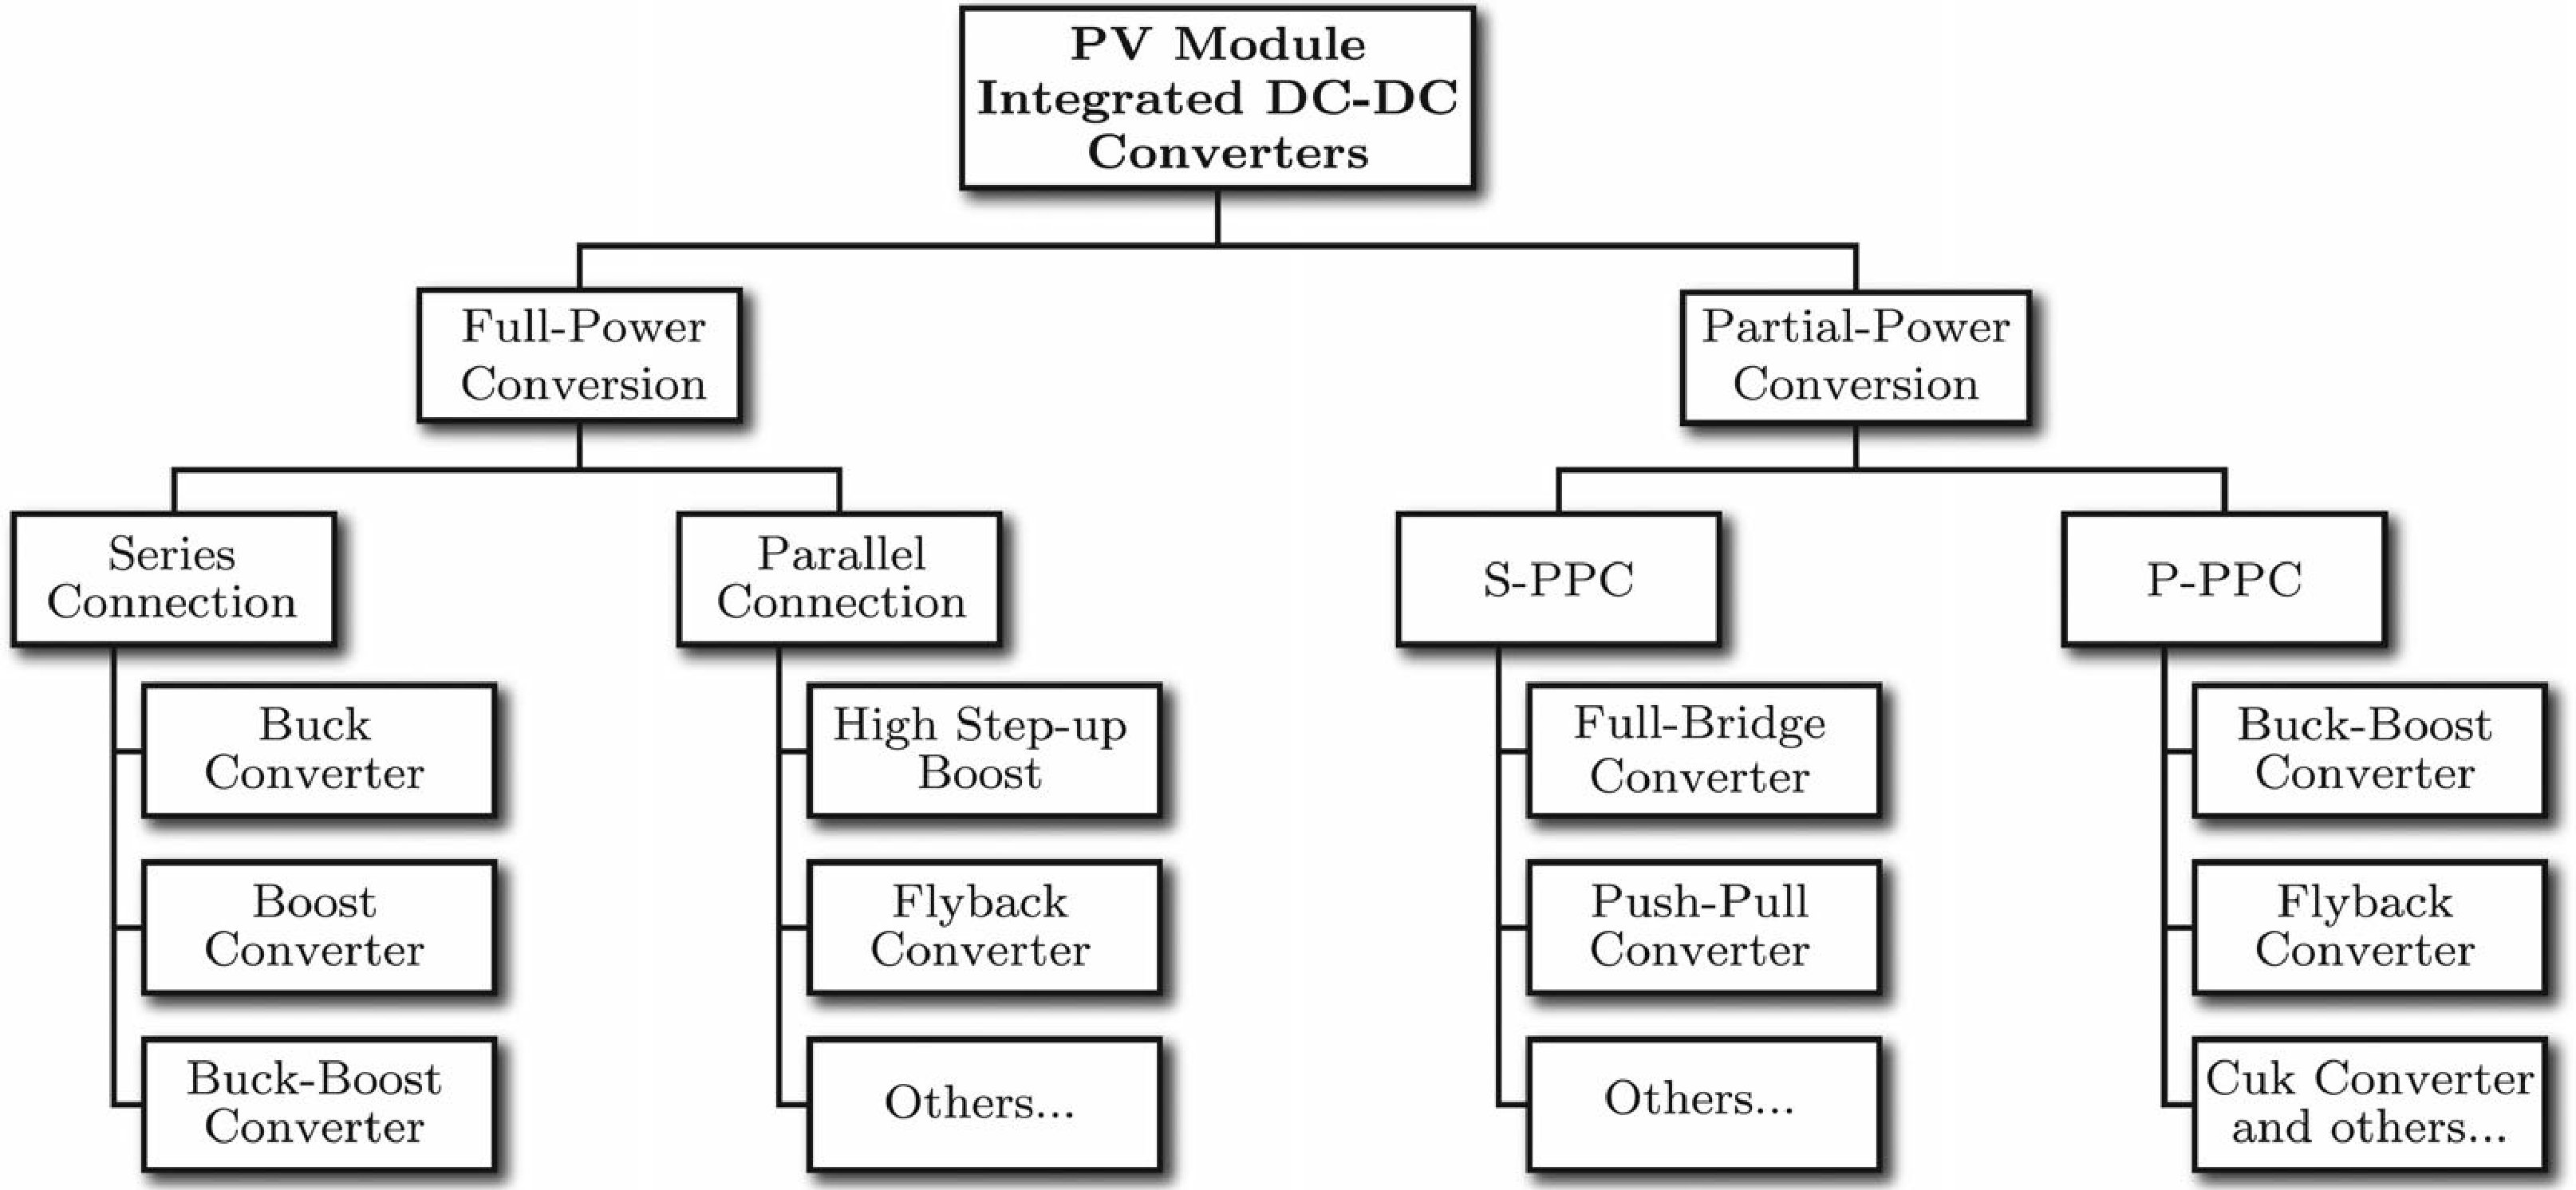
\includegraphics[width=\textwidth, height=0.75\textwidth]{Methodology/fig2.pdf}
        \caption{Subcaption 1}
        \label{fig:subcaption1}
    \end{subfigure}
    \hfill
    \begin{subfigure}[b]{0.48\textwidth}
        \centering
        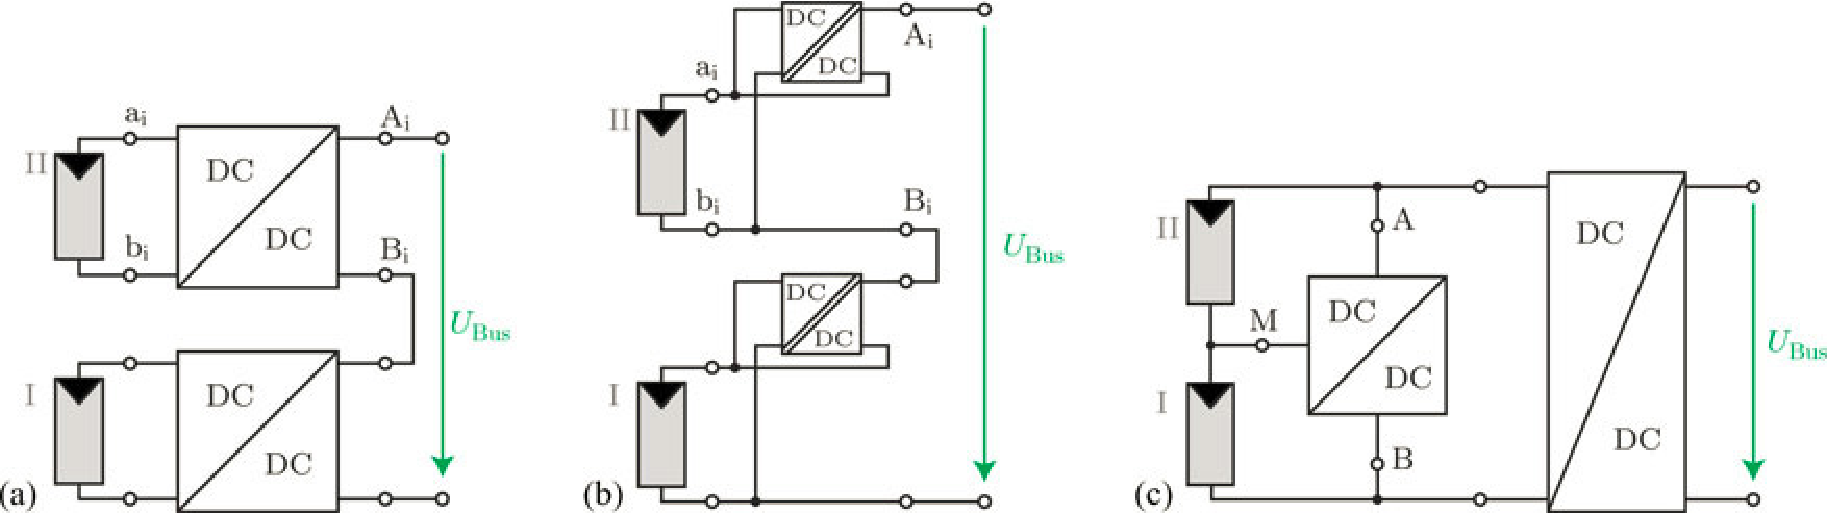
\includegraphics[width=\textwidth, height=0.75\textwidth]{Methodology/fig3.pdf}
        \caption{Subcaption 2}
        \label{fig:subcaption2}
    \end{subfigure}
    \hfill
    \begin{subfigure}[b]{0.48\textwidth}
        \centering
        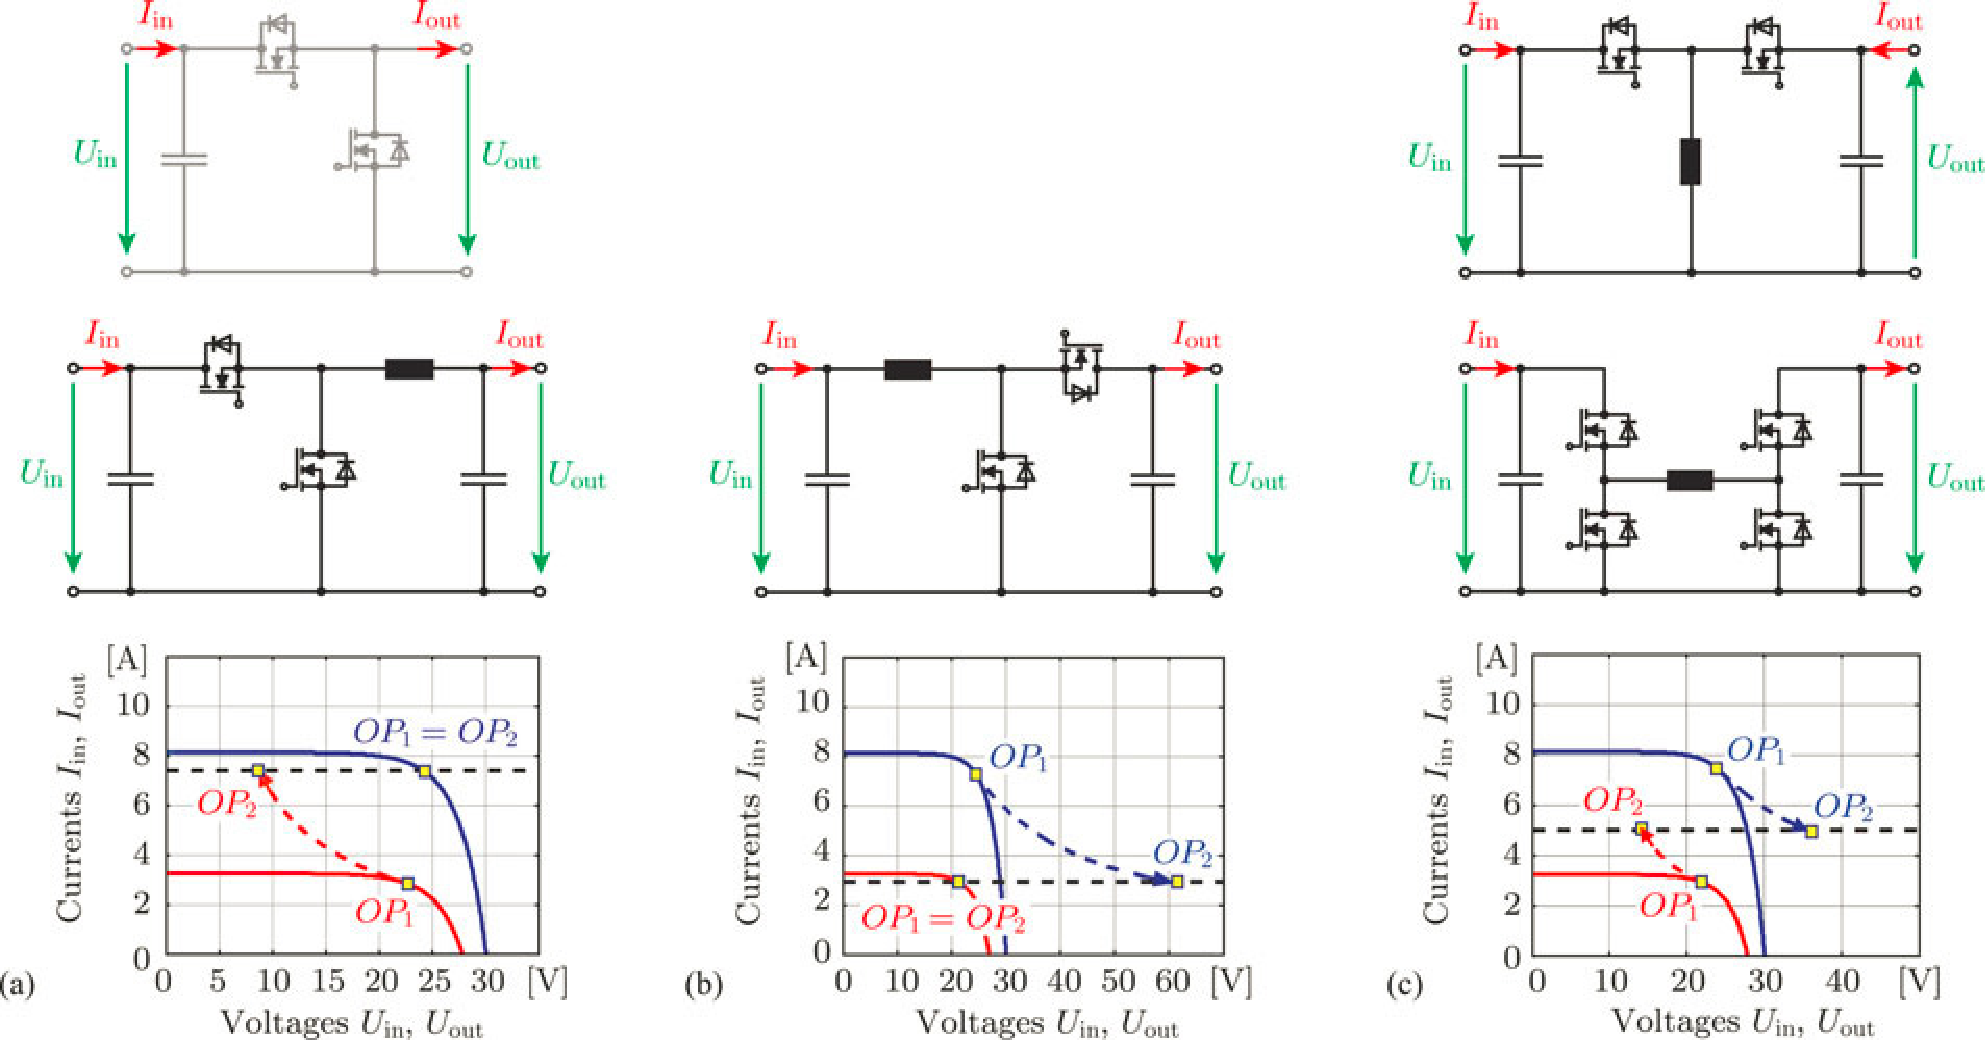
\includegraphics[width=\textwidth, height=0.75\textwidth]{Methodology/fig4.pdf}
        \caption{Subcaption 3}
        \label{fig:subcaption3}
    \end{subfigure}
  \caption{Main caption}
    \label{fig:maincaption}
\end{figure}


